\documentclass{extarticle}
\usepackage[letterpaper, portrait, margin=1in]{geometry} 
\usepackage{tikz}
\usepackage{tikz-qtree}
\usetikzlibrary{shapes}
\usepackage{graphicx}
\usepackage{amsmath}
\usepackage{amsfonts}
\usepackage{amssymb}
\usepackage{amsthm} % theorem package
\usepackage[utf8]{inputenc}
\usepackage{amsthm}
\usepackage{algorithm}
\usepackage[noend]{algpseudocode}
\usepackage[english]{babel}
\theoremstyle{definition}
\newtheorem{theorem}{Theorem}[section]
\theoremstyle{definition}
\newtheorem{definition}{Definition}[section] % define definition

%%% package used by Xiaoli
\usepackage{verbatim}
\usepackage{hyperref}
\usepackage{subfigure}
\usepackage{listings} %% for display code
\usepackage{hyperref} %% add hyperlink
\usepackage{graphicx}
\usepackage{float}




\begin{document}
\title{Homework 2: Texture Synthesis and Image Inpainting \\
	Computer Vision}
\author{Xiaoli He}
\maketitle
\newpage

%%%%%%%%%%%%%%%%%%%%%%%%%%%%%%%%%%%%%%%%%%%%%%%%%%%%%%%%%%%%%%%%%
\section{Texture Synthesis}
The synthesized images for T1,T2,..., T5.gif by with WindowSize = 5, 9,11 pixels are shown in Figure \ref{fig_syth}. The average run time was around s.\\
\begin{figure}[H]
	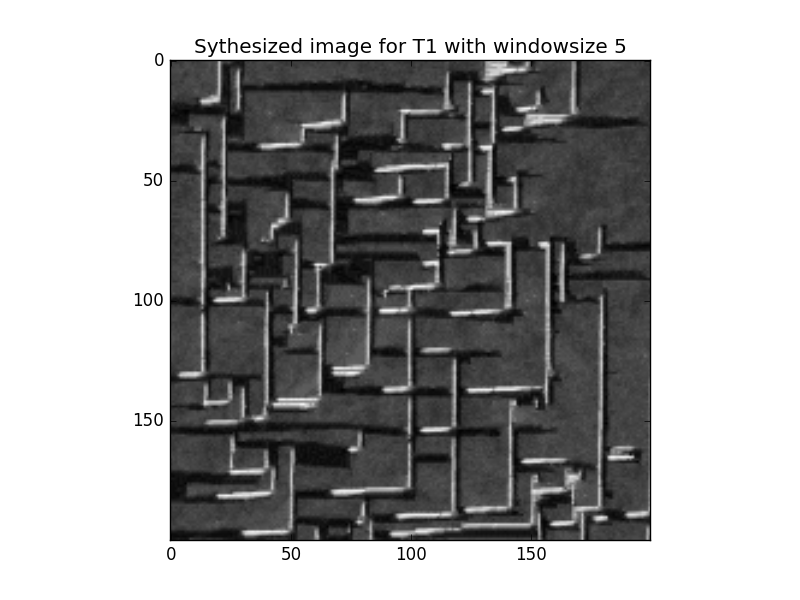
\includegraphics[width = 0.33\textwidth]{./figures/Syth_T1_size_5.png}
	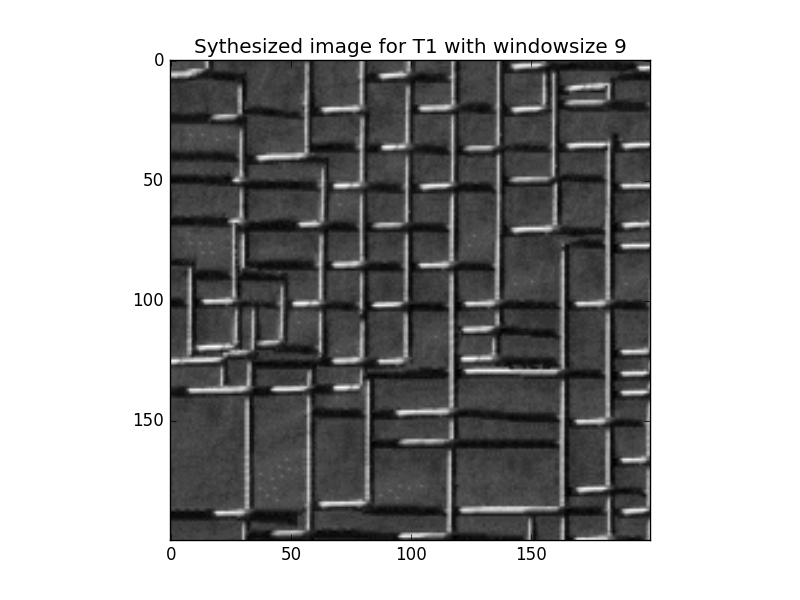
\includegraphics[width = 0.33\textwidth]{./figures/Syth_T1_size_9.png}
	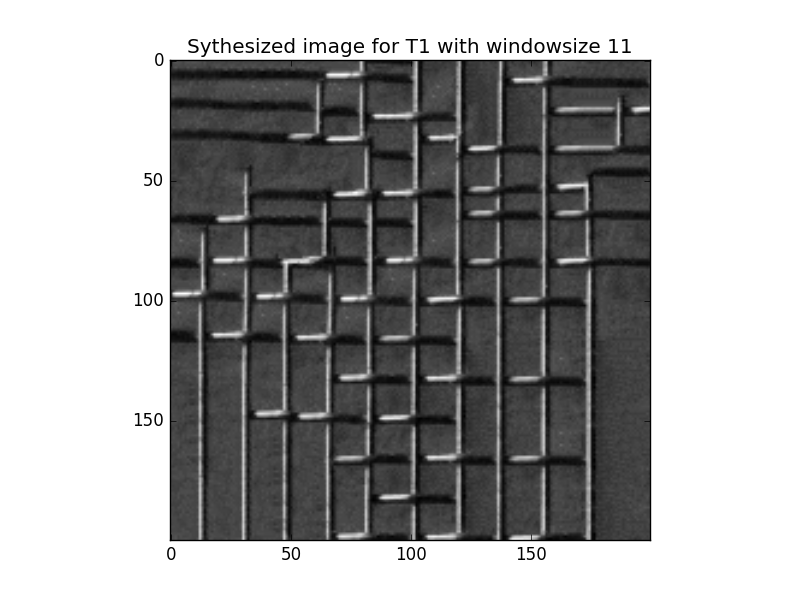
\includegraphics[width = 0.33\textwidth]{./figures/Syth_T1_size_11.png}
	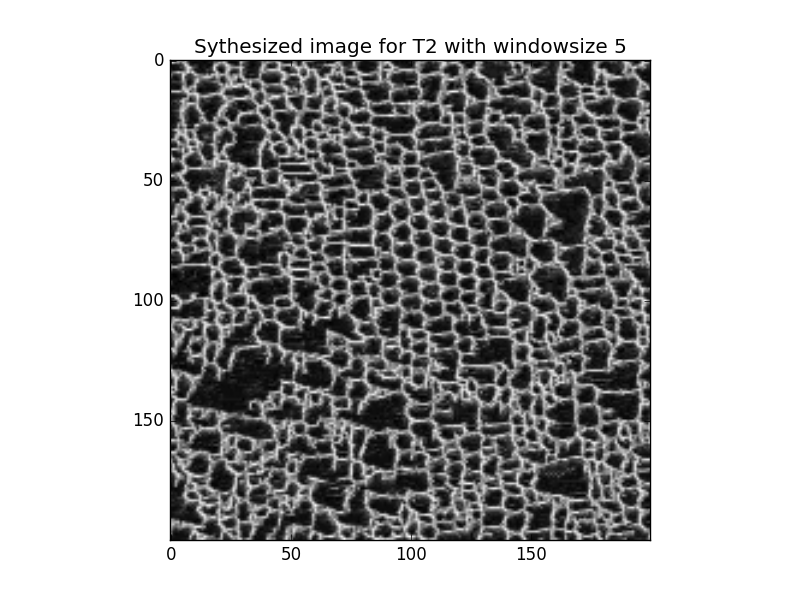
\includegraphics[width = 0.33\textwidth]{./figures/Syth_T2_size_5.png}
	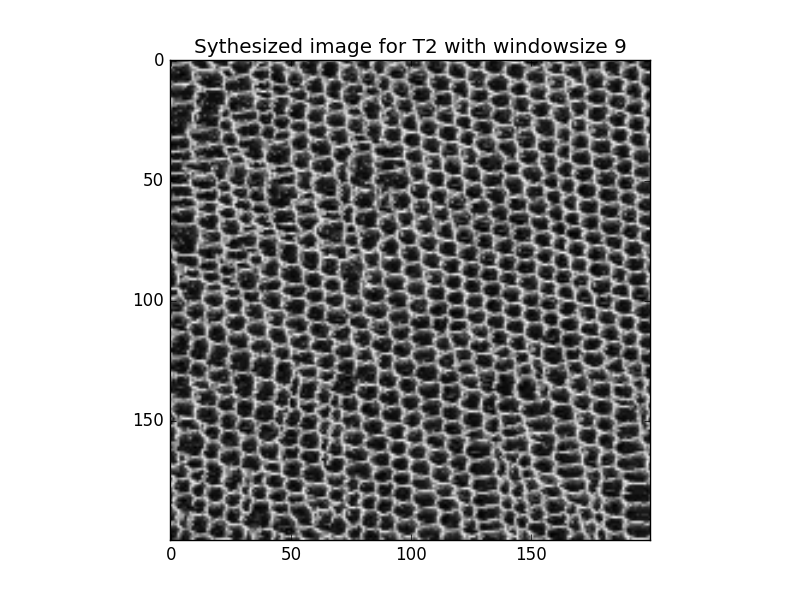
\includegraphics[width = 0.33\textwidth]{./figures/Syth_T2_size_9.png}
	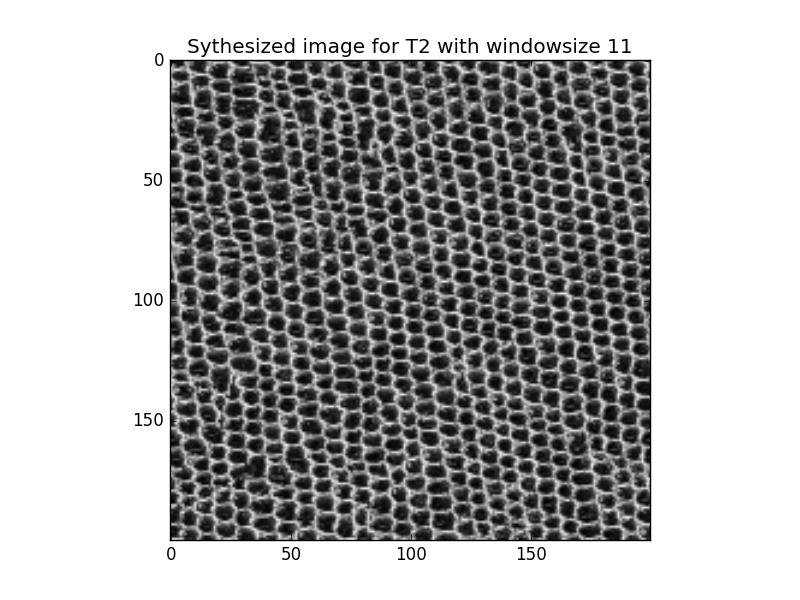
\includegraphics[width = 0.33\textwidth]{./figures/Syth_T2_size_11.png}
	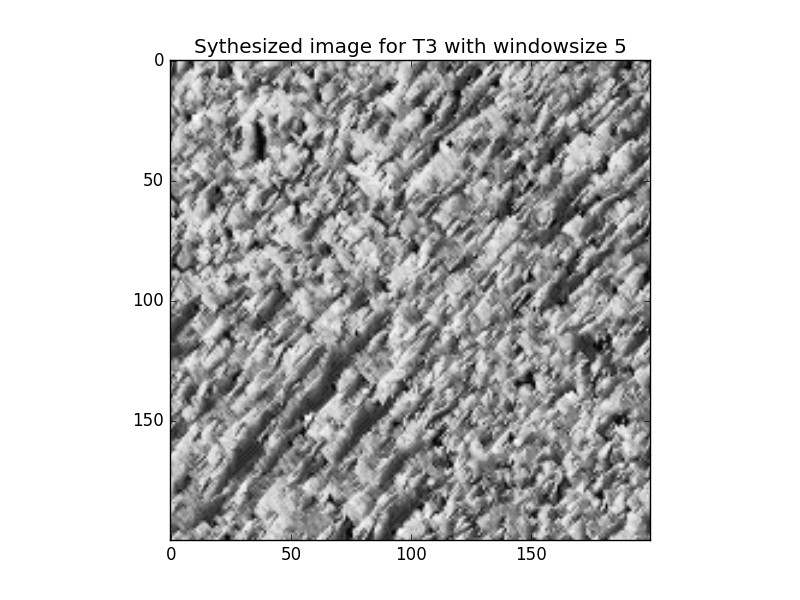
\includegraphics[width = 0.33\textwidth]{./figures/Syth_T3_size_5.png}
	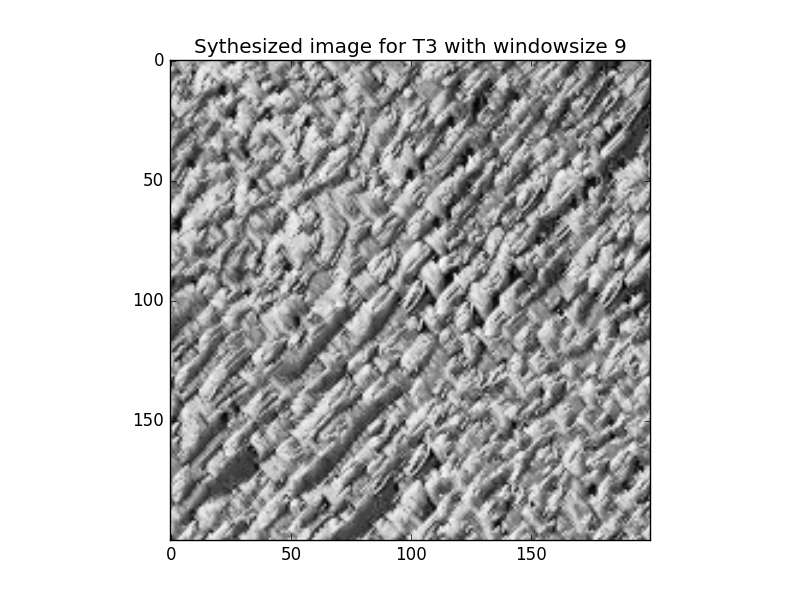
\includegraphics[width = 0.33\textwidth]{./figures/Syth_T3_size_9.png}
	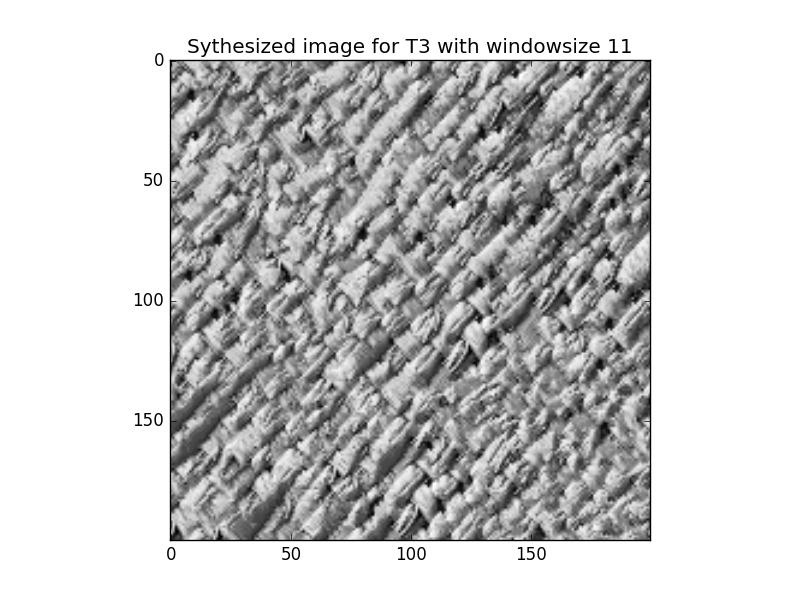
\includegraphics[width = 0.33\textwidth]{./figures/Syth_T3_size_11.png}
	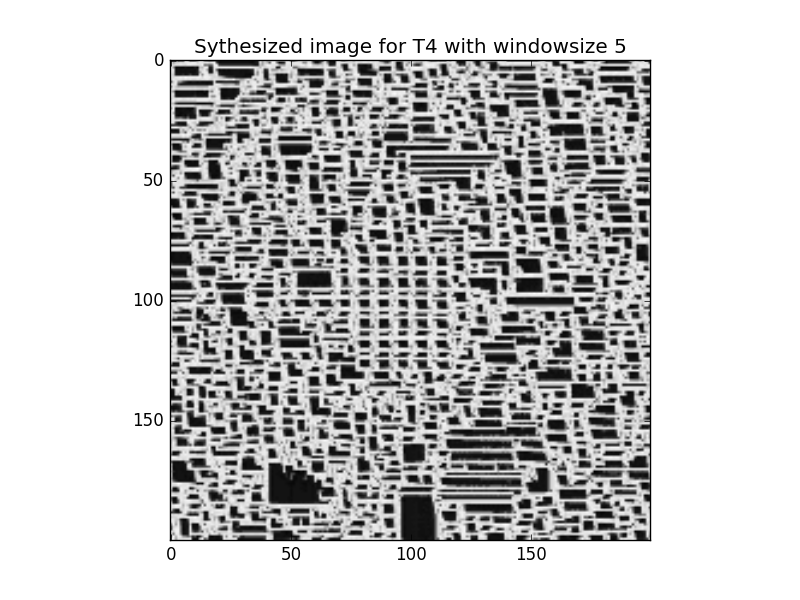
\includegraphics[width = 0.33\textwidth]{./figures/Syth_T4_size_5.png}
	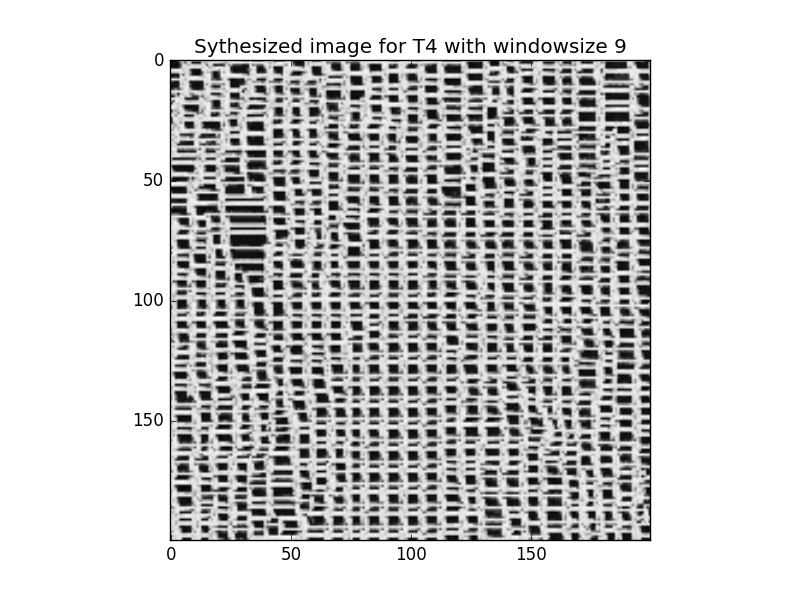
\includegraphics[width = 0.33\textwidth]{./figures/Syth_T4_size_9.png}
	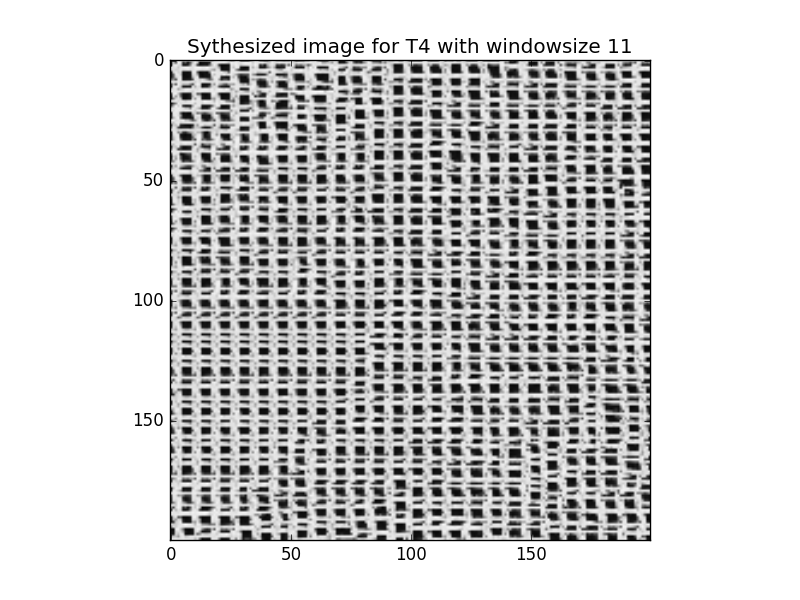
\includegraphics[width = 0.33\textwidth]{./figures/Syth_T4_size_11.png}
	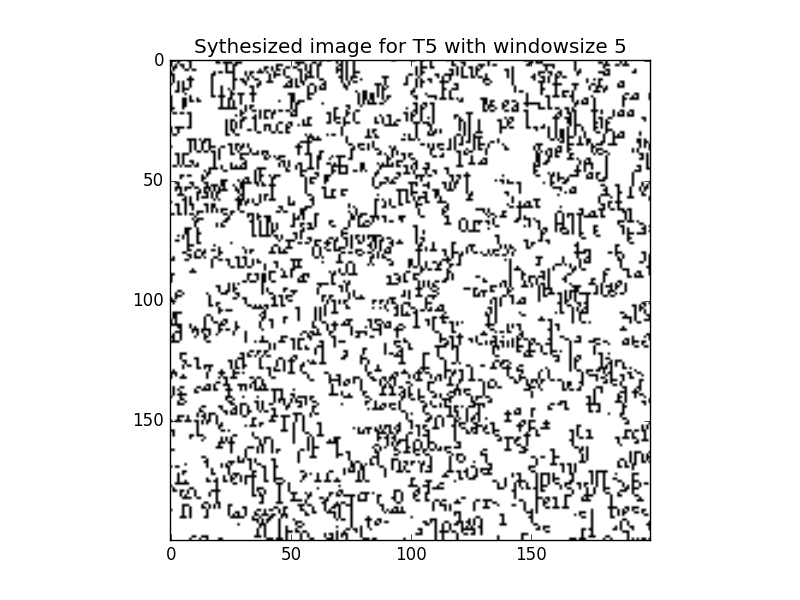
\includegraphics[width = 0.33\textwidth]{./figures/Syth_T5_size_5.png}
	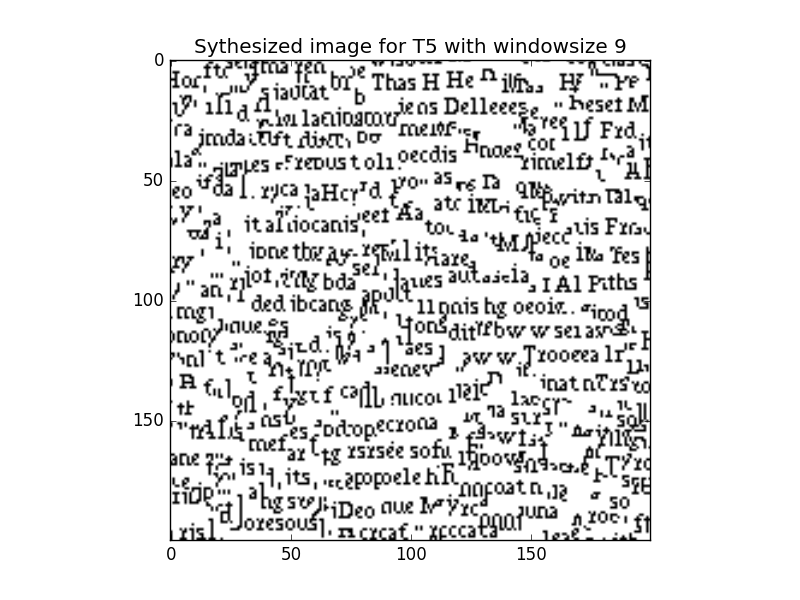
\includegraphics[width = 0.33\textwidth]{./figures/Syth_T5_size_9.png}
	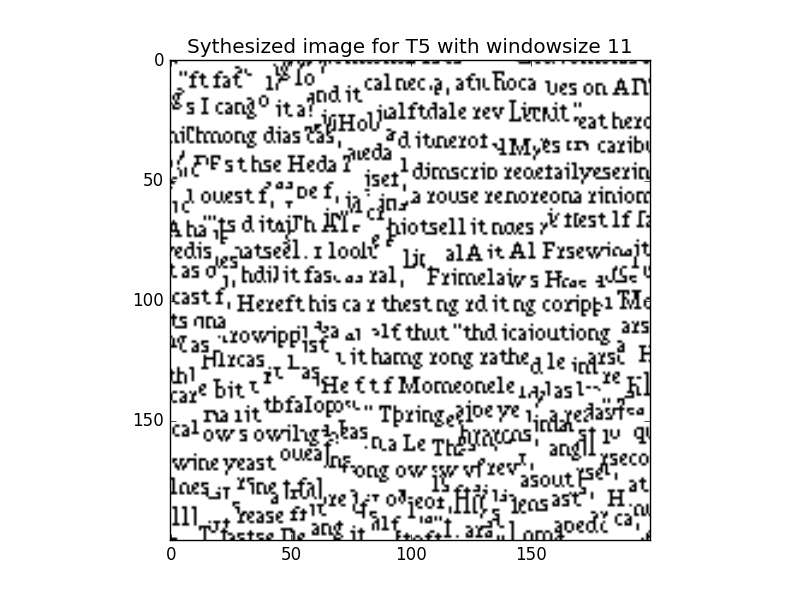
\includegraphics[width = 0.33\textwidth]{./figures/Syth_T5_size_11.png}
	\caption{Synthesized images for T1,T2,T3,T4,T5.gif by with WindowSize = 5, 9,11 pixels}
	\label{fig_syth}
\end{figure}
%%%%%%%%%%%%%%%%%%%%%%%%%%%%%%%%%%%%%%%%%%%%%%%%%%%%%%%%%%%%%%%%%
\section{Image Inpainting}

\pagebreak
\appendix{\textbf{Code files}}\\
Note: to run the codes, you might need to change the directory of:\\
\begin{enumerate}
	\item train.py: (line 14, training image)\\
	\item $test\_xh.py$: (line 14, test image),(line 130,ground truth )\\
	\item RunMyOCRRecogniton.py: (line 13: add current path to sys.path)\\
\end{enumerate}


\textbf{RunMyOCRRecognition:} \\
\lstinputlisting[language=Python]{./code/RunMyOCRRecognition.py}
\pagebreak
\textbf{train:} \\
\lstinputlisting[language=Python]{./code/train.py}
\pagebreak
\textbf{$test\_xh:$} \\
\lstinputlisting[language=Python]{./code/test_xh.py}
\end{document}